\documentclass[12pt]{article}
\usepackage{setspace, graphicx, fullpage, amssymb, amsmath, epsfig, natbib, array, multirow}
\usepackage[bookmarks = false, hidelinks]{hyperref}
\usepackage{amsfonts, bm}
\usepackage{dcolumn}
\usepackage{subfigure, float}
\usepackage[margin=1in]{geometry}
\usepackage{verbatim}
\usepackage{url}
\usepackage{enumerate}
\usepackage{morefloats}
\usepackage[skip = 2pt]{caption}
\usepackage{natbib}
\usepackage[flushleft]{threeparttable}
\usepackage[T1]{fontenc}
\usepackage{libertine}
\usepackage{scrextend}
\usepackage{setspace}
\usepackage{fancyhdr}
\usepackage{enumitem}

\newcommand\fnote[1]{\captionsetup{font=normalsize}\caption*{#1}}

\setlist{nolistsep,noitemsep}
\setlength{\footnotesep}{1.2\baselineskip}
\deffootnote[.2in]{0in}{0em}{\normalsize\thefootnotemark.\enskip}
\newcolumntype{.}{D{.}{.}{-1}}
\newcolumntype{d}[1]{D{.}{.}{#1}}

\makeatother

\renewcommand{\headrulewidth}{0pt}
\def\citeapos#1{\citeauthor{#1}'s (\citeyear{#1})} % possessive citation
\bibpunct{(}{)}{;}{a}{}{,}

\begin{document}

\bibliographystyle{apsr}
\let\OLDthebibliography\thebibliography
% \renewcommand\thebibliography[1]{
%   \OLDthebibliography{#1}
%   \setlength{\parskip}{0pt}
%   \setlength{\itemsep}{1pt}
% }

\title{Party Calls and Reelection in the U.S. Senate%\thanks{
% We would like to thank Andrew Podob for reviewing a draft of this paper.
%ADD FURTHER ACKNOWLEDGEMENTS?
%}
}

% \author{
  % Ethan Hershberger\thanks{
  %   \small Ohio State University
  % }\quad
  % William Minozzi$^\dagger$\quad
  % Craig Volden\thanks{
  %   \small University of Virginia
  % }\\
% }

\date{\today}

\maketitle

\thispagestyle{empty}
\setcounter{page}{0}

\begin{center}

\vspace{.1in}
% Word Count: XXXX
\end{center}
\vspace{.25in}

\begin{abstract}
\singlespacing
\noindent
\cite{Minozzi:2013} advance the idea that a substantial portion of partisan voting activity in Congress is a simple call to unity that is especially easily embraced by ideological extremists.  If correct, their findings should extend from the House to the Senate, despite Senate leaders lacking many of the sticks and carrots found in the House.  We adapt the theory and measurement of party calls to the Senate.  In so doing, we find that both the House and the Senate have relied heavily (and increasingly) on party calls over the past four decades.  In the Senate in particular, the lens of party calls opens new opportunities for scholars to explore partisan legislative behavior.  We take advantage of one such opportunity to show how electoral concerns limit Senators' responsiveness to party calls.
\end{abstract}

\clearpage

\doublespacing

%------------------------------------------------------------------------------%
%------------------------------------------------------------------------------%


\noindent When scholars think of partisan influence in legislative voting they often conceive of pressure exerted on fence-sitting legislators to win them over to the party leaders' preferred position.  Given such a conception, party leaders in the Senate are thought to be less influential than their House counterparts because they possess fewer tools and opportunities to exert pressure.\footnote{\doublespacing\normalsize Yet, recent work has shown significant party effects in the Senate \citep[e.g.,][]{Gailmard:2007, Monroe:2008, Patty:2008, Volden:2006}.}  In contrast with a pressure-based approach to understanding parties, \cite{Minozzi:2013} offer a theory of party calls.  They suggest that, on many issues, unity among party members serves broad partisan ends, such as brand development \citep[e.g.,][]{Snyder:2002}, apart from attempts to win closely contested votes on legislation.  As a result, leaders' attempts to call party members to vote together will be more influential on extremists (who benefit from a coherent brand) than on cross-pressured moderates.  Minozzi and Volden (MV) identify party-call votes and find enhanced responsiveness to them among extremists in the U.S. House.

In this paper, we argue that the logic of party calls extends to the U.S. Senate, even absent strong tools to coerce the institution's individualistic members.  We adapt MV's approach to the Senate and find strong evidence of party calls uniting party members, especially inducing ideological extremists to vote with the rest of the party, above and beyond their natural tendencies.

In addition to extending the examination of party calls to the Senate, we expand the time period of examination from MV to include the 93$^{\text{rd}}$ through the 112$^{\text{th}}$ Congresses (1973-2012) for both the House and the Senate. Consistent with other evidence of partisan polarization across this era, we see a steady rise in the use of party calls over time across both chambers and regardless of Democrat or Republican control. Finally, we argue that extending the study of party calls to the Senate opens numerous opportunities for important new scholarship.  Illustrating one such possibility, we show that Senators up for reelection are significantly less responsive to party calls, consistent with bucking the party when it is out of line with voters in their home states.


%------------------------------------------------------------------------------%
\subsection*{Party Calls in the Senate}
%------------------------------------------------------------------------------%

To explore party calls, MV use a two-step process, first dividing floor votes into ``party-free votes'' and ``party calls,'' and then examining which legislators are most responsive to party calls beyond their baseline partisan support on party-free votes.  Identifying party calls is a difficult classification problem requiring researchers to identify a strong party-based voting pattern apart from that produced by ideological differences alone.  We mimic the approach in MV that produces the list of party-call votes and simultaneously generates party-free ideal points for each legislator.\footnote{\doublespacing\normalsize Minor modifications were made to adapt this method to the Senate and to reduce computational burdens (see Supplemental Appendix A).}

The party calls identified through this process broadly reflect properties expected of partisan votes (see Supplemental Appendix A for details).  For example, party calls tend to drive a further wedge between Democrats and Republicans who are already initially separated on ideological grounds.  Moreover, party calls are more likely to occur among close votes than lopsided votes, perhaps because the close votes offer greater opportunity for parties to differentiate themselves.  In total, these patterns lend confidence that our classification of party-call votes is meaningful in capturing broad and consistent underlying behavior.

\begin{figure}[t]
\centering
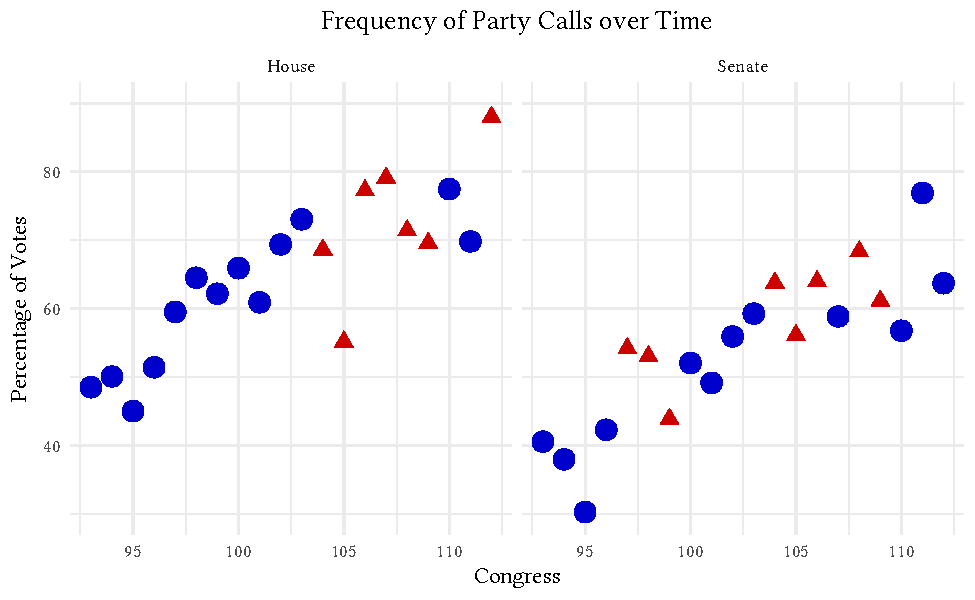
\includegraphics{party_call_percent_both.pdf}
\caption{Party calls as a percentage of all votes, 1973-2012.
This figure shows the percentage of votes classified as party calls per Congress in each chamber. Circles denote Democrat-majority chambers while triangles denote Republican-majority chambers.
\label{fig-party-calls-over-time}}
\end{figure}

Figure~\ref{fig-party-calls-over-time} illustrates the percentage of party calls among all votes in the House and Senate.  Across both chambers, the use of party calls has been steadily increasing over time.\footnote{\doublespacing\normalsize
Differences across chambers based on membership size render
% Because of the different threshold for identifying party calls across chambers, as well as their different membership sizes,
direct House-Senate comparisons in the proportion of party-call votes
%would be
inappropriate.
% do we need to say this?
}  It is possible that parties are calling more because partisan ideological alignment has made party calls more effective, or because parties need members to rally more to get their agendas through a heavily gridlocked Congress.  We believe that the underlying cause of this trend merits further investigation, but take it as consistent with the much discussed increased partisanship and polarization in recent decades \citep[e.g.,][]{Aldrich:2000, Lee:2009, Lee:2016, Theriault:2013, Smith:2014}. This trend holds regardless of which party is in the majority in the chamber.


Fundamental to the theory of party calls is the idea that much partisan activity in Congress works to align members who might otherwise wander away from the party for idiosyncratic reasons, rather than solely winning close votes. As such, those most responsive to party calls are the extremists who benefit from coherent party positions, rather than cross-pressured, fence-sitting moderates.  To test this ``responsive extremists hypothesis,'' we run a series of linear models of \textit{Responsiveness} to party calls, legislator's percentage support for the party position on party-call votes.  Throughout, we cluster observations by legislator and congress to account for possible dependence.  Table~\ref{tab-responsiveness-regressions} shows that the responsive extremists hypothesis holds up well in the extended period over which we examine the House, and nearly as prominently in the Senate.

\begin{table}[!htbp]
\centering
\begin{threeparttable}
\caption{Models of \textit{Responsiveness}, 1973-2012}
\label{tab-responsiveness-regressions}
\singlespacing
\begin{tabular}{l c c c }
\hline
& House & \multicolumn{2}{c}{Senate} \\
\hline

Ideological Extremism & $7.75^{***}$ & $6.29^{***}$ & $6.23^{***}$  \\
                      & $(1.26)$     & $(0.82)$     & $(0.82)$      \\
Baseline Rate         & $0.57^{***}$ & $0.73^{***}$ & $0.74^{***}$  \\
                      & $(0.12)$     & $(0.07)$     & $(0.07)$      \\
Up For Reelection     &              &              & $-0.95^{***}$ \\
                      &              &              & $(0.19)$      \\
Vote Share            & $-0.01$      & $0.03$       & $0.03$        \\
                      & $(0.03)$     & $(0.03)$     & $(0.03)$      \\
Pres Vote Share       & $0.03$       & $0.10$       & $0.10$        \\
                      & $(0.08)$     & $(0.05)$     & $(0.05)$      \\
Leader                & $1.81^{**}$  & $1.64^{*}$   & $1.63^{*}$    \\
                      & $(0.56)$     & $(0.72)$     & $(0.72)$      \\
Chair                 & $4.98^{***}$ & $2.13^{**}$  & $2.10^{**}$   \\
                      & $(0.95)$     & $(0.79)$     & $(0.79)$      \\
Power Committee       & $2.76^{***}$ & $-0.67$      & $-0.67$       \\
                      & $(0.76)$     & $(0.71)$     & $(0.72)$      \\
Best Committee        & $-0.17$      & $0.16$       & $0.16$        \\
                      & $(0.10)$     & $(0.14)$     & $(0.14)$      \\
Female                & $1.17$       & $2.05^{*}$   & $2.03^{*}$    \\
                      & $(0.63)$     & $(0.88)$     & $(0.89)$      \\
African American      & $1.90$       & $-4.58$      & $-4.69$       \\
                      & $(1.36)$     & $(2.49)$     & $(2.46)$      \\
Latino                & $3.27^{**}$  & $5.60^{*}$   & $5.66^{*}$    \\
                      & $(1.16)$     & $(2.54)$     & $(2.52)$      \\
South                 & $-0.89$      & $0.60$       & $0.60$        \\
                      & $(0.54)$     & $(0.70)$     & $(0.70)$      \\
Seniority             & $-0.05$      & $0.01$       & $0.01$        \\
                      & $(0.06)$     & $(0.07)$     & $(0.07)$      \\
Freshman              & $0.78$       & $1.08^{*}$   & $0.80$        \\
                      & $(0.67)$     & $(0.54)$     & $(0.56)$      \\
Intercept             & $31.78^{**}$ & $11.67$      & $11.90$       \\
                      & $(11.77)$    & $(6.93)$     & $(6.90)$      \\
\hline
R$^2$                 & 0.46         & 0.63         & 0.63          \\
Adj. R$^2$            & 0.46         & 0.63         & 0.63          \\
Num. obs.             & 8544         & 1991         & 1991          \\
RMSE                  & 8.44         & 6.98         & 6.97          \\
\hline

\end{tabular}
\begin{tablenotes}
   \item
   The table presents linear models of \textit{Responsiveness} to Party Calls,
   from the 93$^{\text{rd}}$-112$^{\text{th}}$ Congresses (1973-2012).
  Standard errors are clustered by Congress and member.\\
   $^{***}p<0.001$, $^{**}p<0.01$, $^*p<0.05$
 \end{tablenotes}
\end{threeparttable}
\end{table}

% didn't MV include retiree?
We include the control variables from MV, notably accounting for the \textit{Baseline Rate} of voting with the party on party-free votes.\footnote{\doublespacing\normalsize See Supplemental Appendix B for descriptions and summary statistics for all variables.}  Although some House-Senate differences emerge, such as for Southerners or those on power committees, the broad patterns are consistent across institutions.\footnote{\doublespacing\normalsize Given the small size of the Senate, most members are on one of the top committees, limiting the variance that allowed patterns based on committee assignments to be discerned in the House.}  For example, positive coefficients show \textit{Party Leaders} and \textit{Committee Chairs} to be highly responsive to party calls.

As shown by the coefficients on \textit{Ideological Extremism} and in strong support of the theory of party calls, each one standard deviation increase in that variable is associated with a nearly eight percentage point increase in \textit{Responsiveness} in the House, and more than six points in the Senate.\footnote{\doublespacing\normalsize The effect sizes are similar with those uncovered by MV in the House between 1973 and 2006.}  This party alignment extends above and beyond the baseline support on party-free votes.

The pattern of ideological extremists being more responsive to party calls than moderates holds for both Democrats and Republicans, for both those in the majority party and those in the minority party (see Supplemental Appendix C for details). This robust support is illustrated in Figure~\ref{fig-extremism-responsiveness} based on separate regressions for each party in each Congress, which is a tough test of the responsive extremists hypothesis, especially given the small membership of the Senate. In the House, \textit{Ideological Extremism} takes a positive coefficient for all but four cases, and in the Senate for all but two. Further, in the House, all positive coefficients are statistically significant; in the Senate, 29 of the 38 positive coefficients are statistically significant, while only one negative coefficient is. These results add confidence to the aggregate findings above.

\begin{figure}[t]
\centering
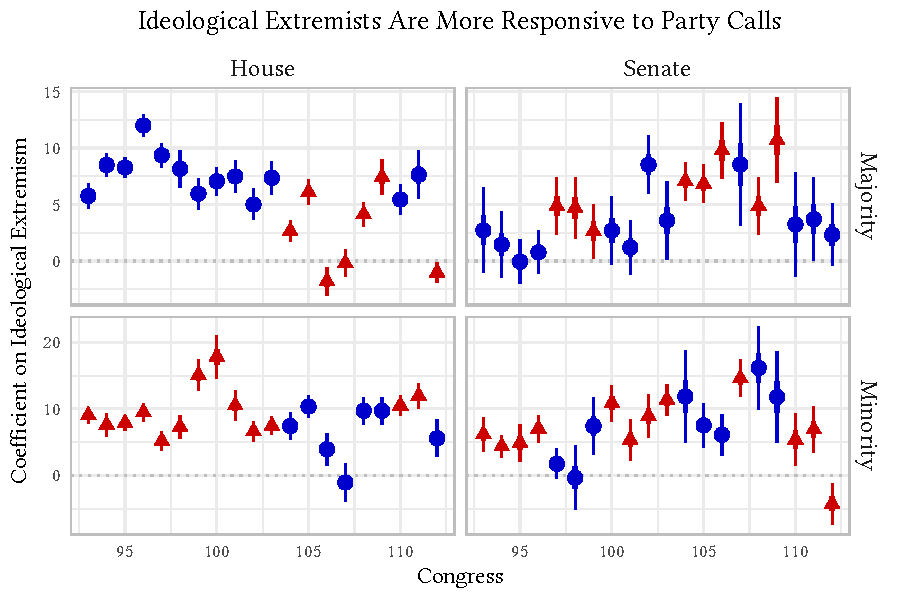
\includegraphics{both-chambers-figure2.pdf}
\caption{Extremists are responsive to party calls in both chambers.
This coefficient plot is produced by the same formula shown in the House and Senate regression table with results decomposed for the majority and minority parties in each of the 93$^{\text{rd}}$-112$^{\text{th}}$ Congresses (1973-2012).
Circles denote Democrat-majority chambers while triangles denote Republican-majority chambers, and both indicate coefficient estimates for \textit{Ideological Extremism} in regressions of \emph{Responsiveness} to party calls, with both 50\% and 95\% confidence intervals shown.
\label{fig-extremism-responsiveness}}
\end{figure}

These results paint a coherent portrait of party calls in both chambers of the U.S. Congress. Party-call votes are widespread, have increased over the past four decades, and divide Democrats from Republicans. But most importantly, these votes draw \emph{ideologically extreme} members---rather than moderates---toward the unified partisan position.

Beyond uncovering such a systematic and important partisan process in Congress, the party calls identified here offer the potential to significantly enhance scholarly exploration of parties in the Senate. New research based on party calls could contribute to a fuller understanding of partisan practices and norms spreading from the House to the Senate \citep[e.g.,][]{Theriault:2013}, of the role of partisanship in advancing and overcoming filibusters \citep[e.g.,][]{Wawro:2004}, and of electoral constraints on partisan behavior \citep[e.g.,][]{Levitt:1996}, to name a few opportunities.

To illustrate the usefulness of party calls, we tackle the last of these possibilities. Specifically, in the final column of Table~\ref{tab-responsiveness-regressions}, we include an indicator variable for whether a Senator is in her final Congress before reelection.  Based on the theory of party calls, we expect Senators to be more free to help develop a party brand, even in contrast to their constituents' preferences, when electoral threats are close behind them rather than when the next election is imminent.  Consistent with this hypothesis, Table~\ref{tab-responsiveness-regressions} shows about one percentage point lower responsiveness to party calls among those \textit{Up for Reelection} than among those in their first four years following an election, all else equal.  In the next section, we explore this result more fully.

%------------------------------------------------------------------------------%
\subsection*{Reelection Limits Responsiveness to Party Calls}
%------------------------------------------------------------------------------%

We argue that Senators up for reelection will be more attuned to their electoral needs than to broad party interests. Put simply, they will use some party-call votes to improve their personal---rather than the party---brand
\citep[e.g.,][]{Canes-Wrone:2002, Carson:2010}.  We detected evidence consistent with such a pattern above, but as a more targeted test, we build a design on same-state Senator pairs in which one Senator is \textit{Up for Reelection} at the end of the Congress.  These pairings are ideal because same-state Senators are elected by the same constituents, but not at the same time, allowing us to estimate the effects of being \textit{Up for Reelection} using a model with fixed effects for each state-Congress pair.  We further control for all relevant covariates and adjust for lagged \textit{Ideological Extremism}, \textit{Responsiveness}, and \textit{Baseline Rate}. Similar results hold if these control variables are omitted (see Supplemental Appendix D).
%Given this design, any additional differences apart from reelection between members from the same state should cancel each other out across Senators and over time, limiting the possibility of spuriously significant findings.
% not sure I think this is right...
Based on the logic above, we expect that the Senator \textit{Up for Reelection} will be have lower \textit{Responsiveness} to party calls than her same-state Senate partner.  In contrast, we expect no difference between the \textit{Baseline Rate} of voting with the party on party-free votes, which therefore comprises a test of our design. See Supplemental Appendix D for details.

\begin{figure}[t]
\centering

\includegraphics[width = 12cm]{senate_difference_estimates.pdf}

\caption{Senators up for reelection are less responsive to party calls, yet there is no evidence that reelection affects \textit{Baseline Rate} of voting with the party.  This figure summarizes fixed effects models of same-state Senator pairs in which one is \textit{Up for Reelection}.  Estimates are differences in \textit{Responsiveness} to party calls and the \textit{Baseline Rate} of voting with the party, with 50\% and 95\% confidence intervals based on clustered standard errors.
\label{fig-reelection-responsiveness}}
\end{figure}

Figure~\ref{fig-reelection-responsiveness} shows that \textit{Responsiveness} to party calls declines an average of about 1.3\% when a Senator is \textit{Up for Reelection}.  However, their \textit{Baseline Rate} of voting with the party is unchanged by electoral considerations,
an anticipated null finding that bolsters our confidence in the validity of this research design.\footnote{\doublespacing\normalsize  In an alternative approach, we compared all three possibilities for same-state Senator pairs based on proximity to upcoming election.  Comparing those \textit{Up for Reelection} to those in the first Congress after election shows a similar effect to that in Figure~\ref{fig-reelection-responsiveness}.  Likewise, comparing those \textit{Up for Reelection} to those in the middle two years of their six-year term reveals lower \textit{Responsiveness} for those \textit{Up for Reelection}.  In contrast, comparing same-state Senators neither of whom are \textit{Up for Reelection}, we find no difference in \textit{Responsiveness}, treating the more senior Senator as the one closer to election.  Across all three cases, we find no differences in their \textit{Baseline Rate}.}
% which serves to validate our design insofar as such an effect was unexpected and inconsistent with the party calls theory.
During the period of analysis, the average \textit{Responsiveness} to party calls is 85\%. Across the 365 party-call votes in the average Senate, a Senator not \textit{Up for Reelection} therefore averages 53 defections from her party.  In contrast, those \textit{Up for Reelection} defect from party calls 58 times on average, almost a ten percent increase.  Such deviations may limit the party's effectiveness in both lawmaking and brand development.  But they offer the election-seeking Senator an opportunity to build her support and reputation back home.

\subsection*{Conclusion}

In this paper, we established that legislators respond to party calls in the Senate as they do in the House. In both chambers, party calls have become more prominent over the past forty years.  In line with expectations, when leaders issue party calls, legislators align with their party, with the greatest effect being among ideological extremists.

One especially noteworthy finding is the nature of the relationship we uncover between party and ideology.  In contrast to \citeapos{Krehbiel:1993} view that partisanship is often merely a reflection of ideology, or \citeapos{Lee:2009} view that party extends well beyond ideology, we find party and ideology to be largely complementary yet distinct.  When the party calls its members together, those who benefit the most---typically ideological extremists---respond most vigorously to the call.

We further showed the value of party calls as a tool for studying legislative behavior.  We found that reelection reduced member responsiveness to party calls.  Under electoral threat, constituent preferences are front and center in Senators' minds, and thus we hypothesized---and found---that members up for reelection are less responsive to the party. This finding shows one of the limits to the party-building efforts inherent in party calls.

%------------------------------------------------------------------------------%
\bibliography{senate}
%------------------------------------------------------------------------------%

\end{document}
